\documentclass[default]{beamer}
\setbeamertemplate{navigation symbols}{}

\usetheme{CambridgeUS}
\useoutertheme{infolines}
%\usecolortheme{crane}

\usepackage{cmap}							% Поддержка поиска русских слов в PDF (pdflatex)
\usepackage[utf8]{inputenc}					% Выбор языка и кодировки
\usepackage[english, russian]{babel}
\usepackage{csquotes}

\usepackage[
	language=auto,
	autolang=other,
	backend=biber,
	style=authortitle,
	sorting=ydnt
]{biblatex}
\addbibresource{aha.bib}
				
\DeclareSourcemap{
	\maps[datatype=bibtex, overwrite]{
		\map{
			\step[fieldset=langid, fieldvalue=english]
			\step[fieldset=doi, null]
			\step[fieldset=issn, null]
			\step[fieldset=isbn, null]
			\step[fieldset=url, null]
			\step[fieldsource=language, fieldset=langid, origfieldval]
		}
	}
}


\graphicspath{{../../images/}} 			% Пути к изображениям

\makeatletter
\setbeamertemplate{footline}
{
	\leavevmode%
	\hbox{%
		\begin{beamercolorbox}[wd=.333333\paperwidth,ht=2.25ex,dp=1ex,center]{author
				in head/foot}%
			\usebeamerfont{author in
				head/foot}\insertshortauthor~~\beamer@ifempty{\insertshortinstitute}{}{(\insertshortinstitute)}
		\end{beamercolorbox}%
		\begin{beamercolorbox}[wd=.333333\paperwidth,ht=2.25ex,dp=1ex,center]{title in
				head/foot}%
			\usebeamerfont{title in head/foot}\insertshorttitle
		\end{beamercolorbox}%
		\begin{beamercolorbox}[wd=.333333\paperwidth,ht=2.25ex,dp=1ex,right]{date in
				head/foot}%
			\usebeamerfont{date in head/foot}\insertshortdate{}\hspace*{2em}
			\insertframenumber{}\hspace*{2ex} 
		\end{beamercolorbox}
	}%
	\vskip0pt%
}


\renewcommand*{\bibfont}{\tiny}
\setlength\bibitemsep{-5pt}

\begin{document}
	
	\title[Модель картины мира]{Модель картины мира}
	\author[Панов]{Александр Панов}
	\institute[ИСА РАН]{ИСА РАН}
	\date{14 февраля 2018~г.} 
	
	\begin{frame}
		\titlepage
	\end{frame}
		
	\begin{frame}
		%\frametitle{Цели курса}
		\tiny
		\begin{columns}
			\begin{column}{0.6\textwidth}
				
				\begin{columns}
					\begin{column}{0.4\textwidth}
						\begin{center}
							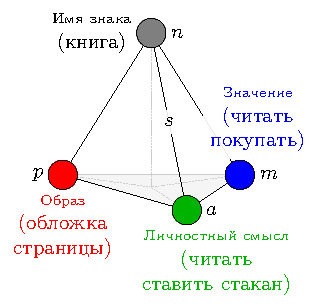
\includegraphics[width=\textwidth]{signs/ru/sign_color_book_ru}
						\end{center}
						
					\end{column}
					\begin{column}{0.6\textwidth}
						Трехкомпонентная структура подтверждается психологическими (Выготский, Леонтьев) и нейрофизиологическими (Иваницкий, Дехане, Гроссберг) работами.
					\end{column}
				\end{columns}
					\textbf{{\scriptsize Формализация}}
						\begin{columns}
							\begin{column}{0.5\textwidth}
								\begin{itemize}
								\item \textit{Синтаксический уровень}: функции связывания, типы отношений на множестве компонент, семиотическая сеть, синтаксические модели.
								\item \textit{Семантический уровень}: множество признаков и правил.
								\item \textit{Структурный уровень}: каузальные матрицы, каузальные сети, структурные модели.
							\end{itemize}
							\end{column}
							\begin{column}{0.5\textwidth}
								\begin{center}
									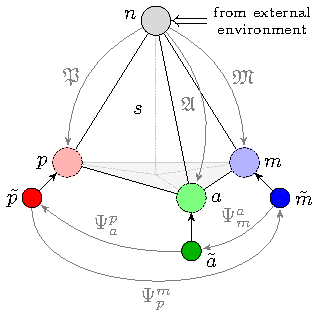
\includegraphics[width=0.5\textwidth]{signs/en/sign_naming_colored_en}
									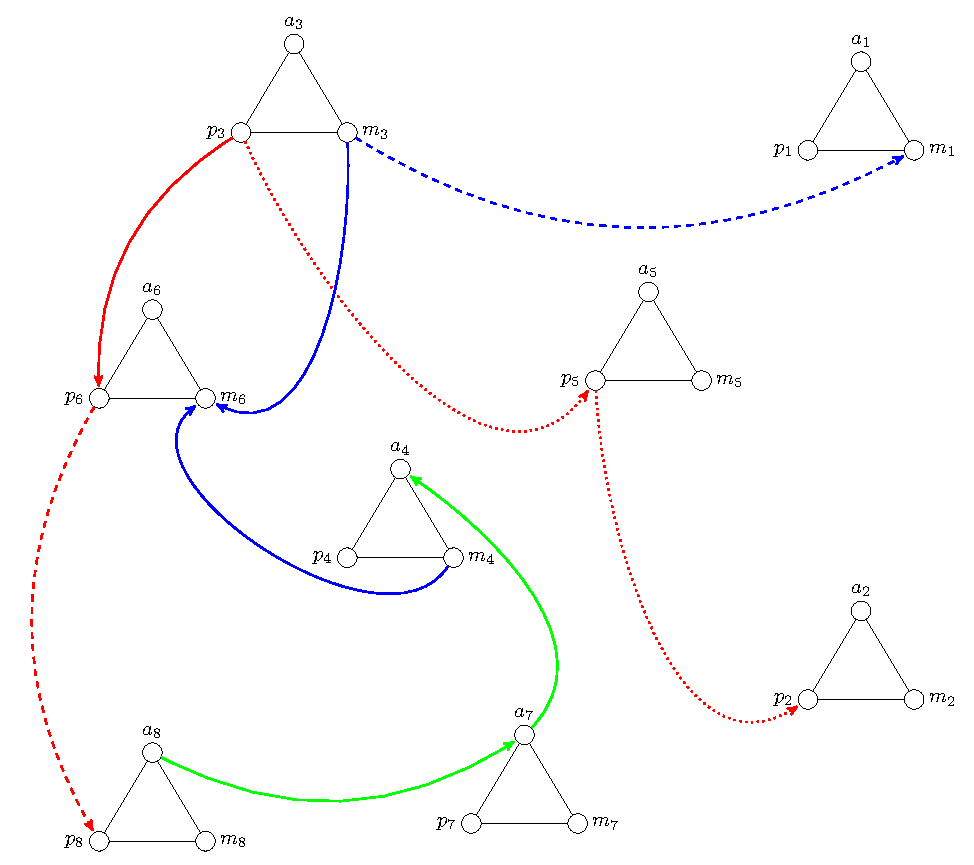
\includegraphics[width=0.5\textwidth]{signnet/signs_net}
									
									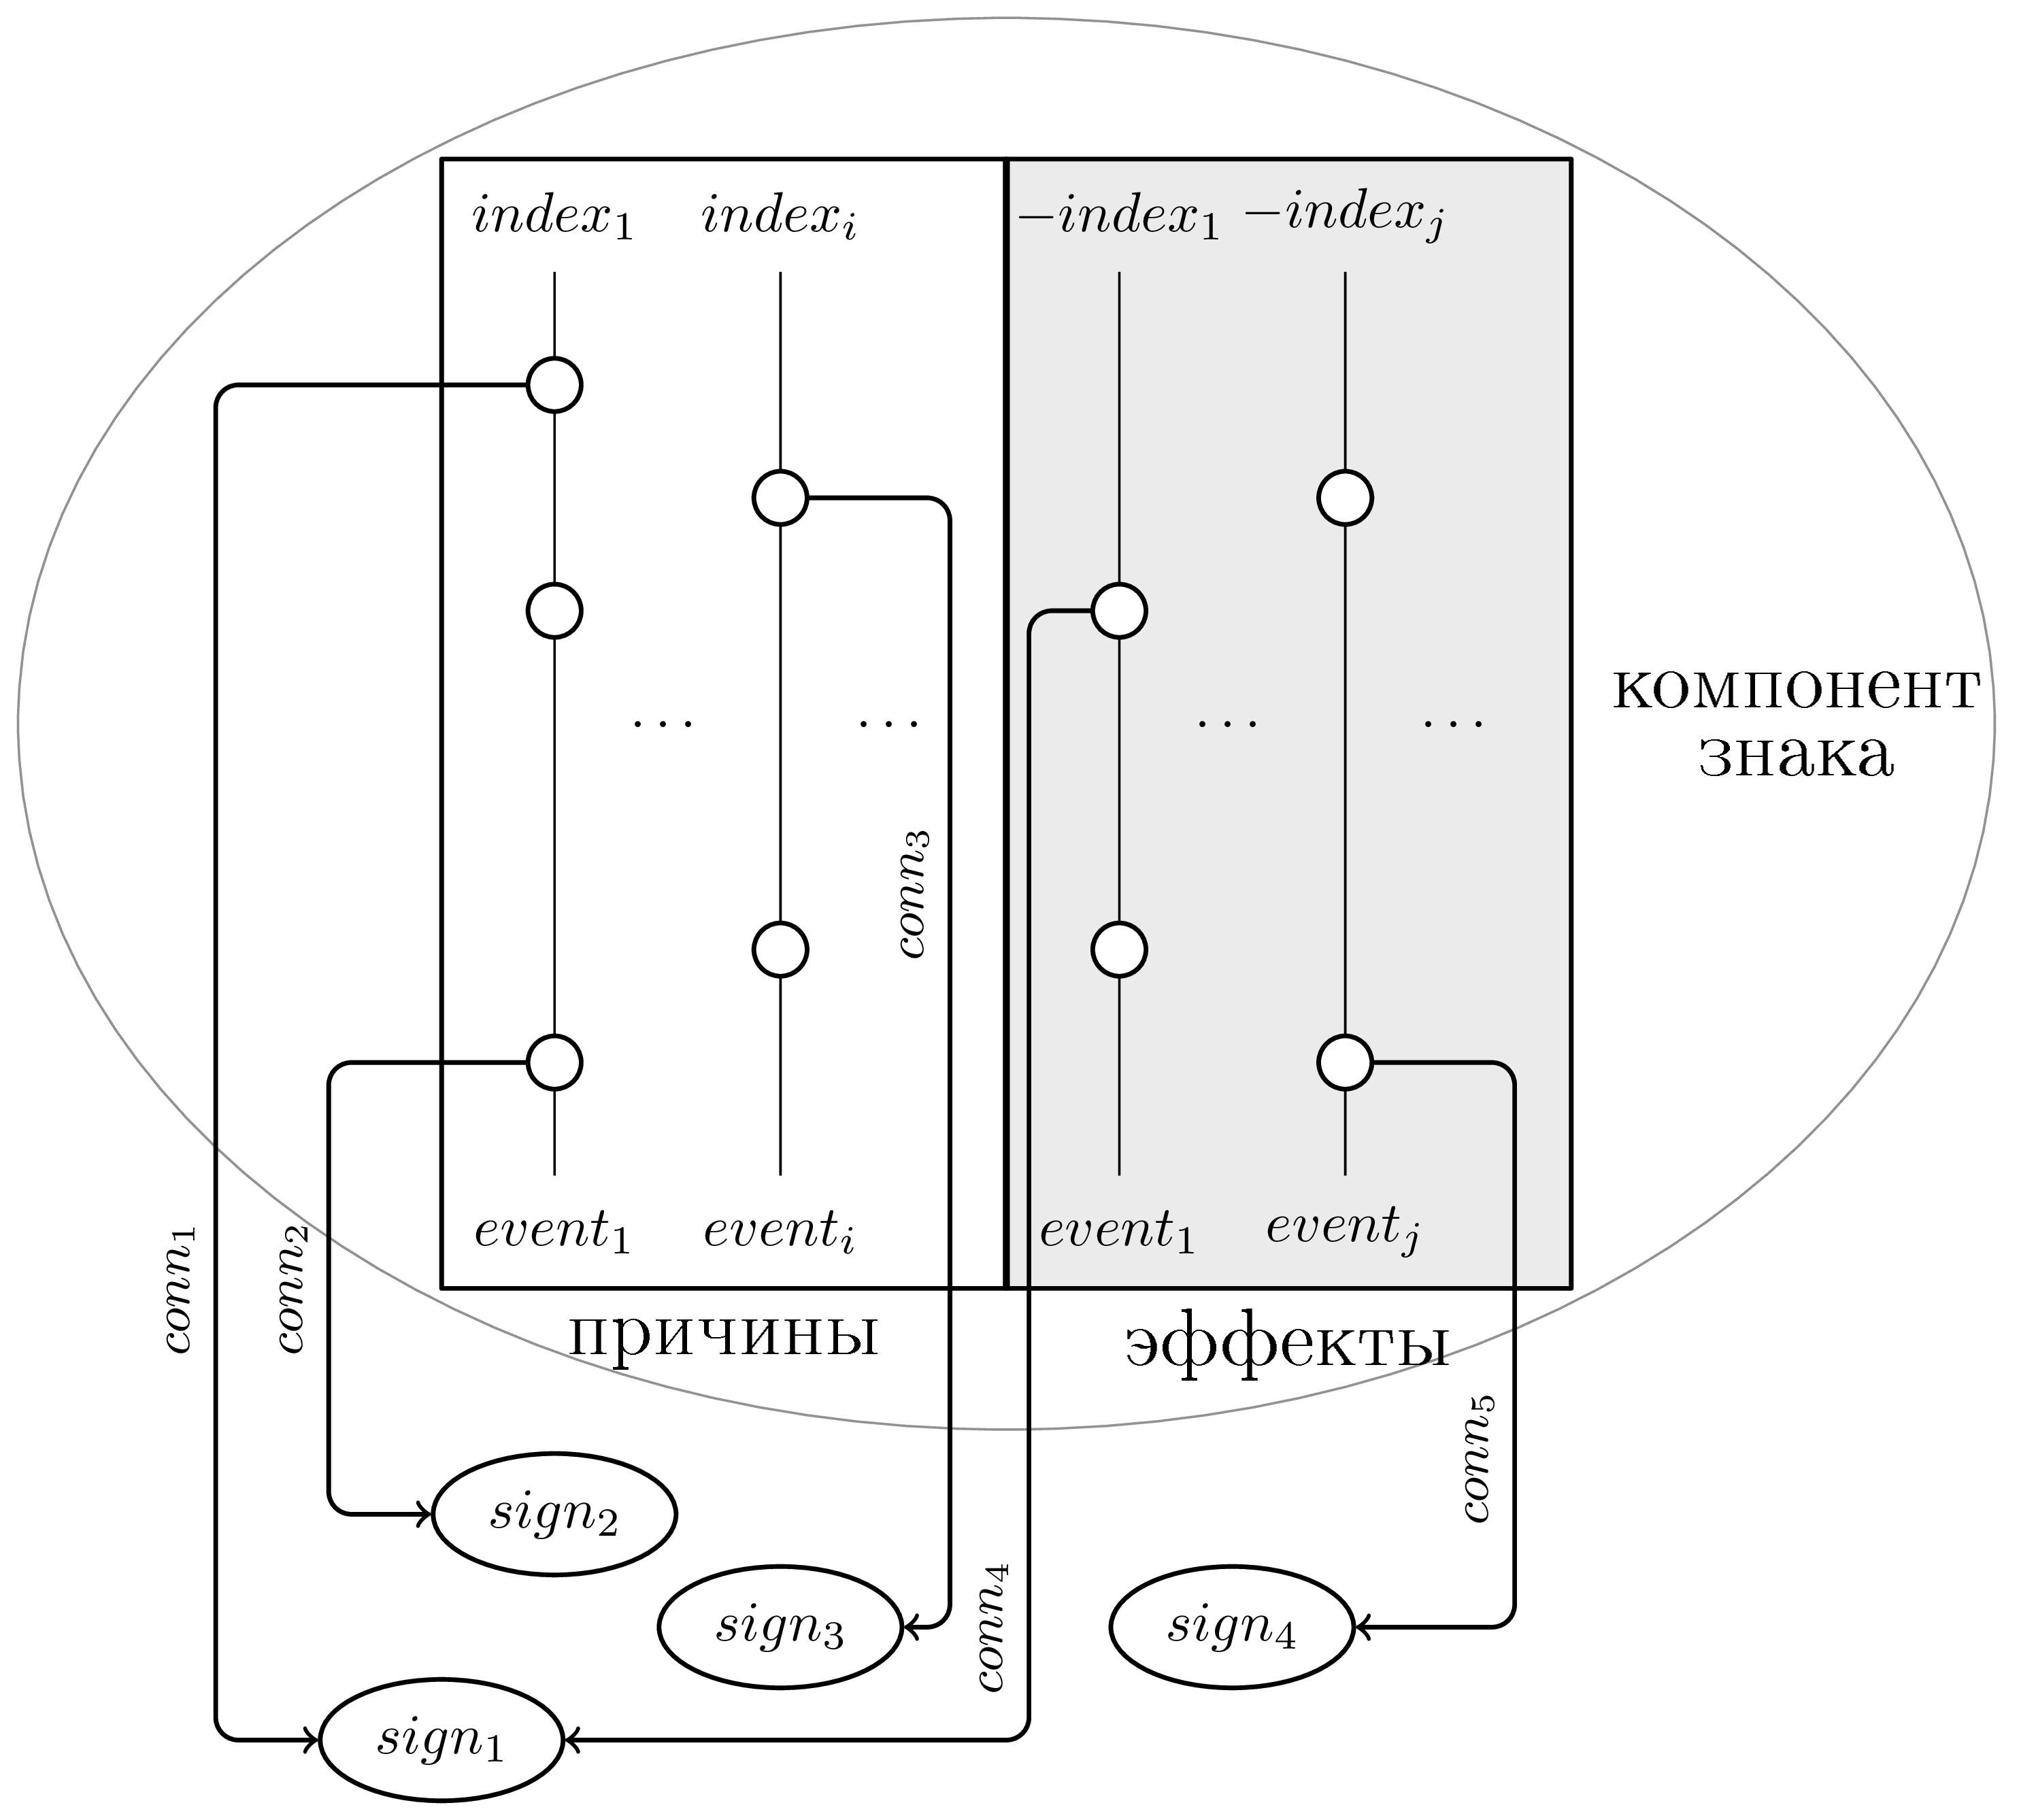
\includegraphics[width=0.5\textwidth]{causnet/caus_matr_ru}
									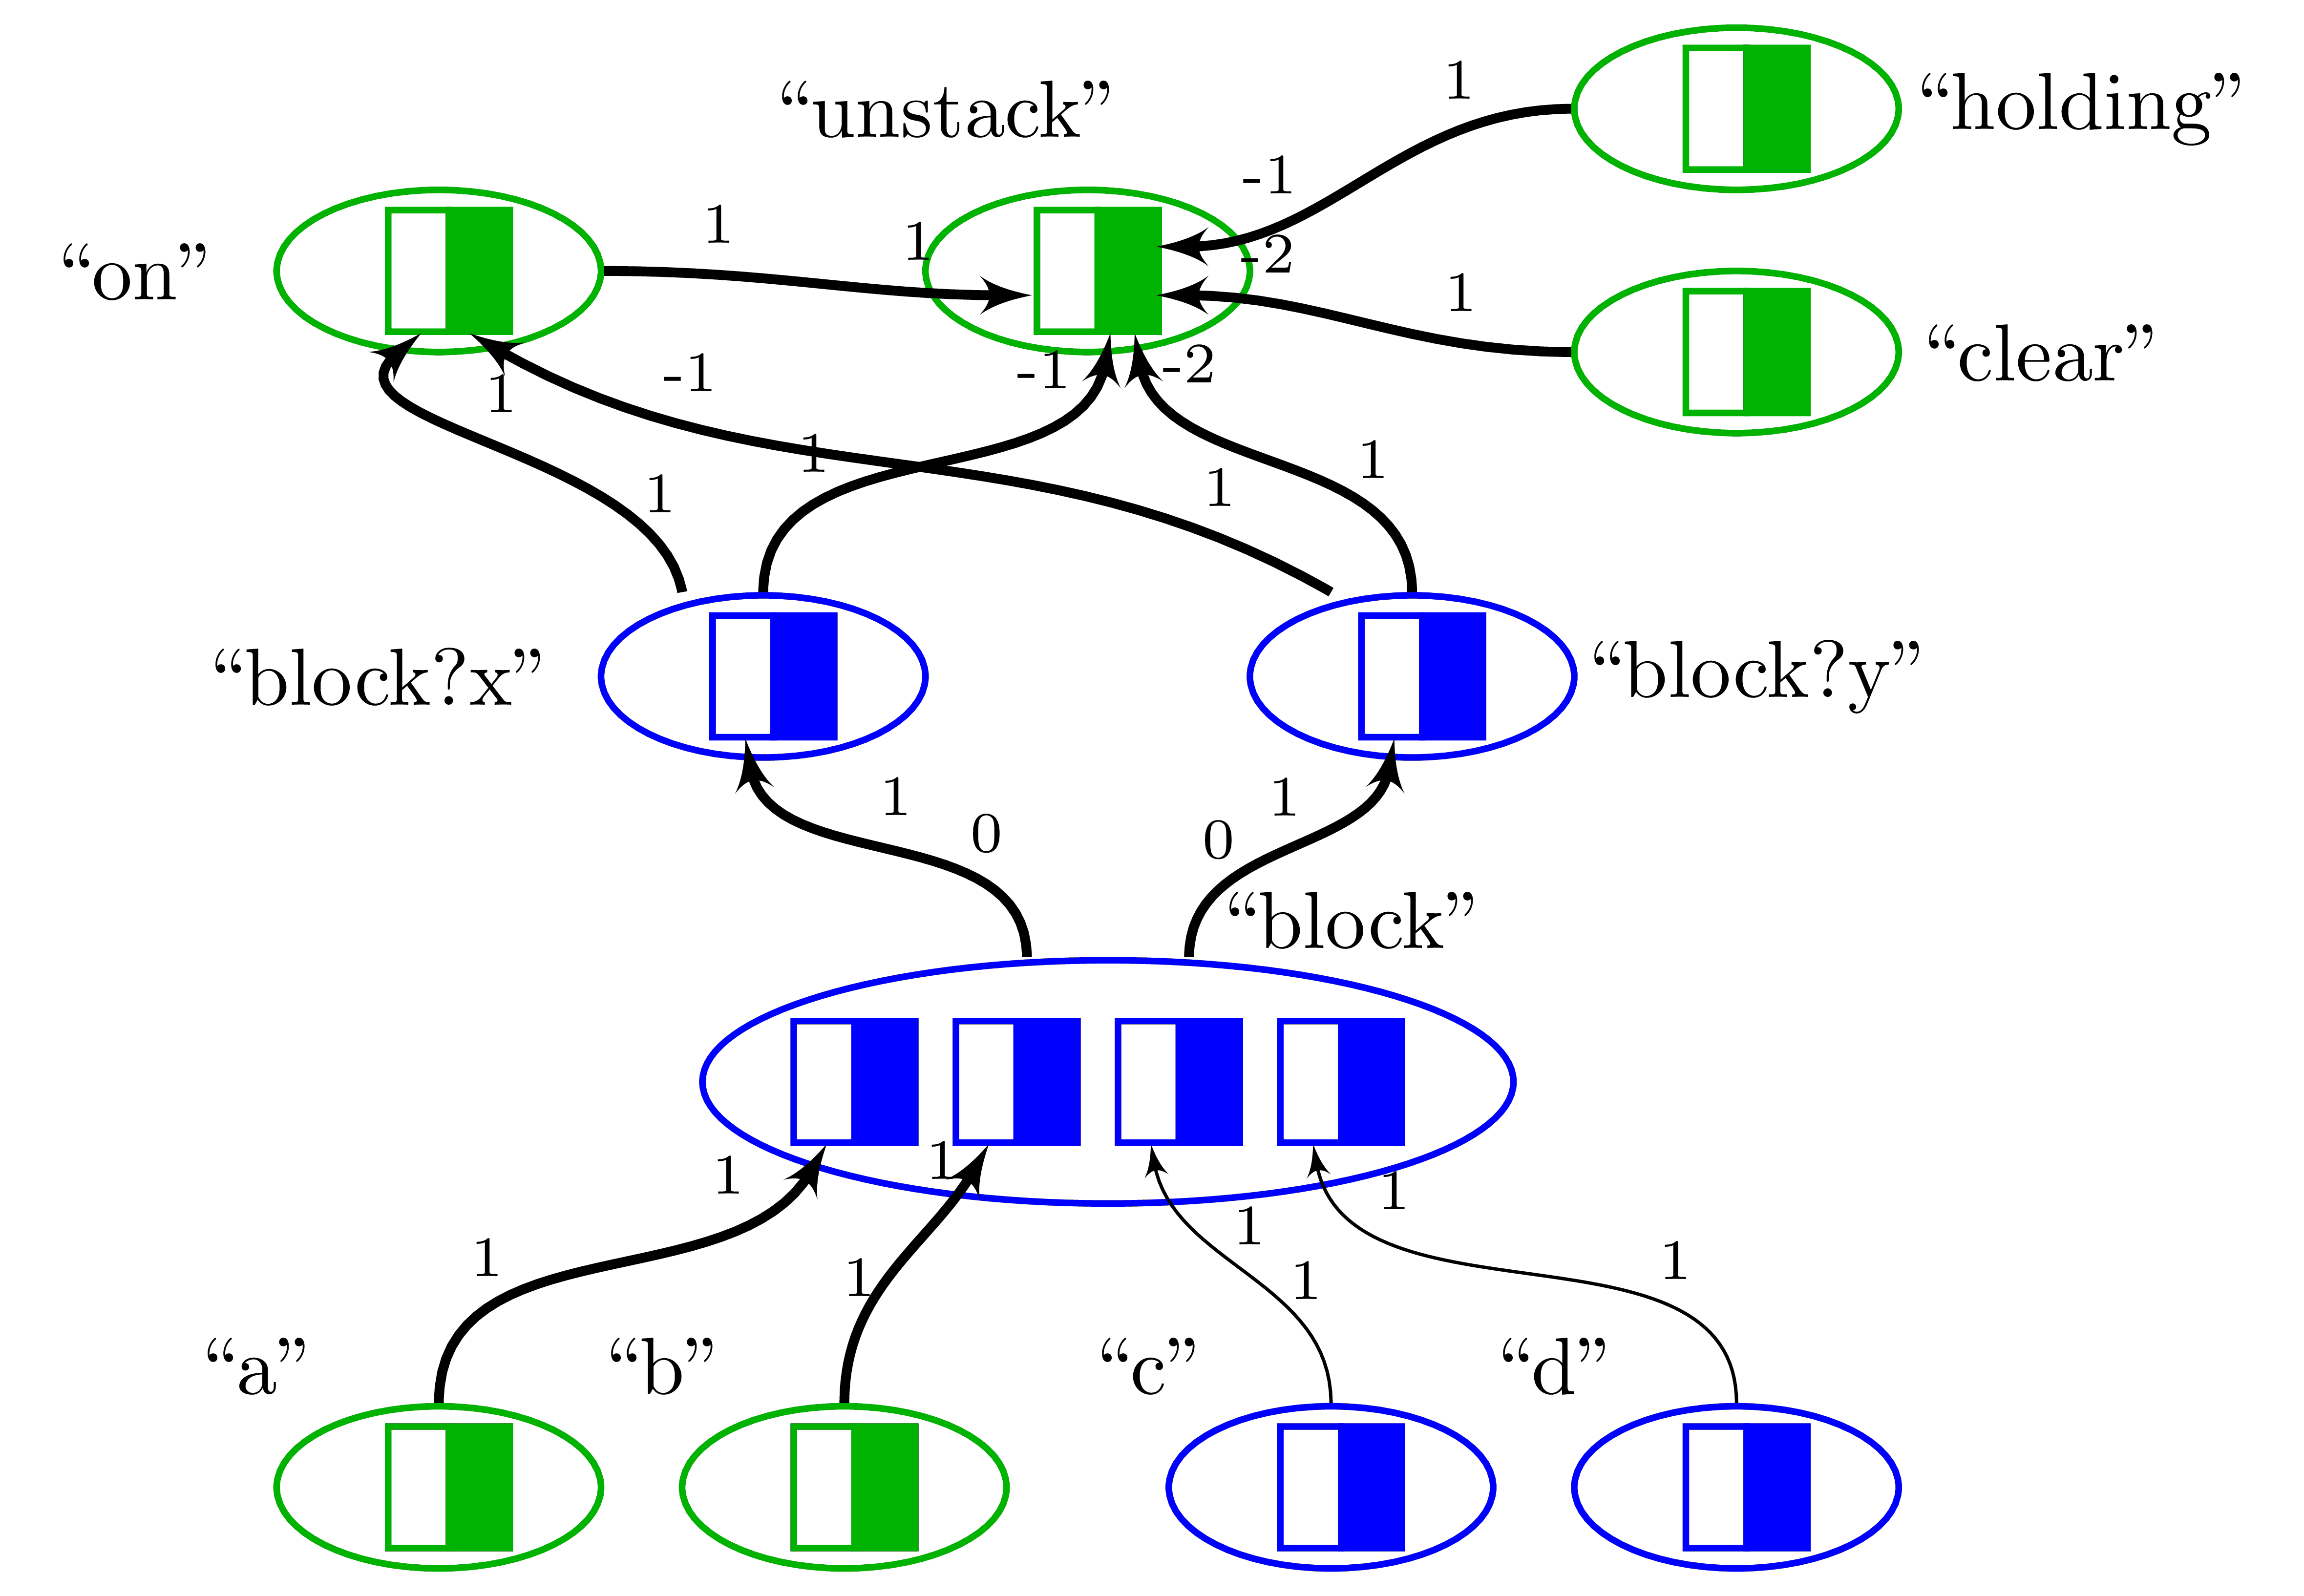
\includegraphics[width=0.5\textwidth]{examples/plan/plan_nets-3}
								\end{center}
							\end{column}
						\end{columns}
			\end{column}
			\begin{column}{0.4\textwidth}
				\textbf{{\scriptsize Моделирование}}
				\begin{itemize}
					\item Распознавание и категоризация.
					\begin{center}
						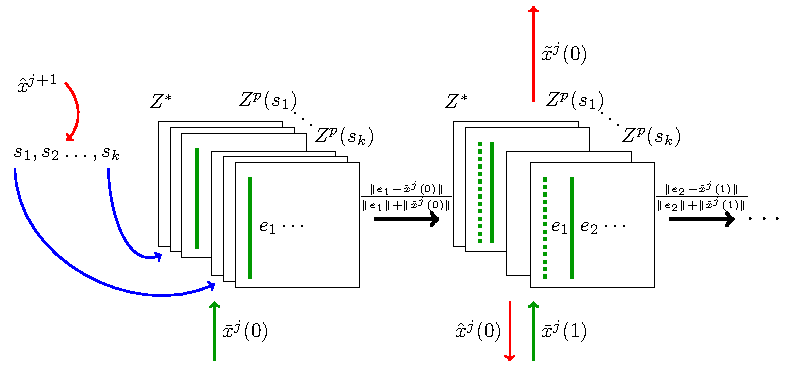
\includegraphics[width=0.6\textwidth]{algo/perception}
					\end{center}
					\item Образование нового знака.
					\item Планирование индивидуального поведения.
					\begin{center}
						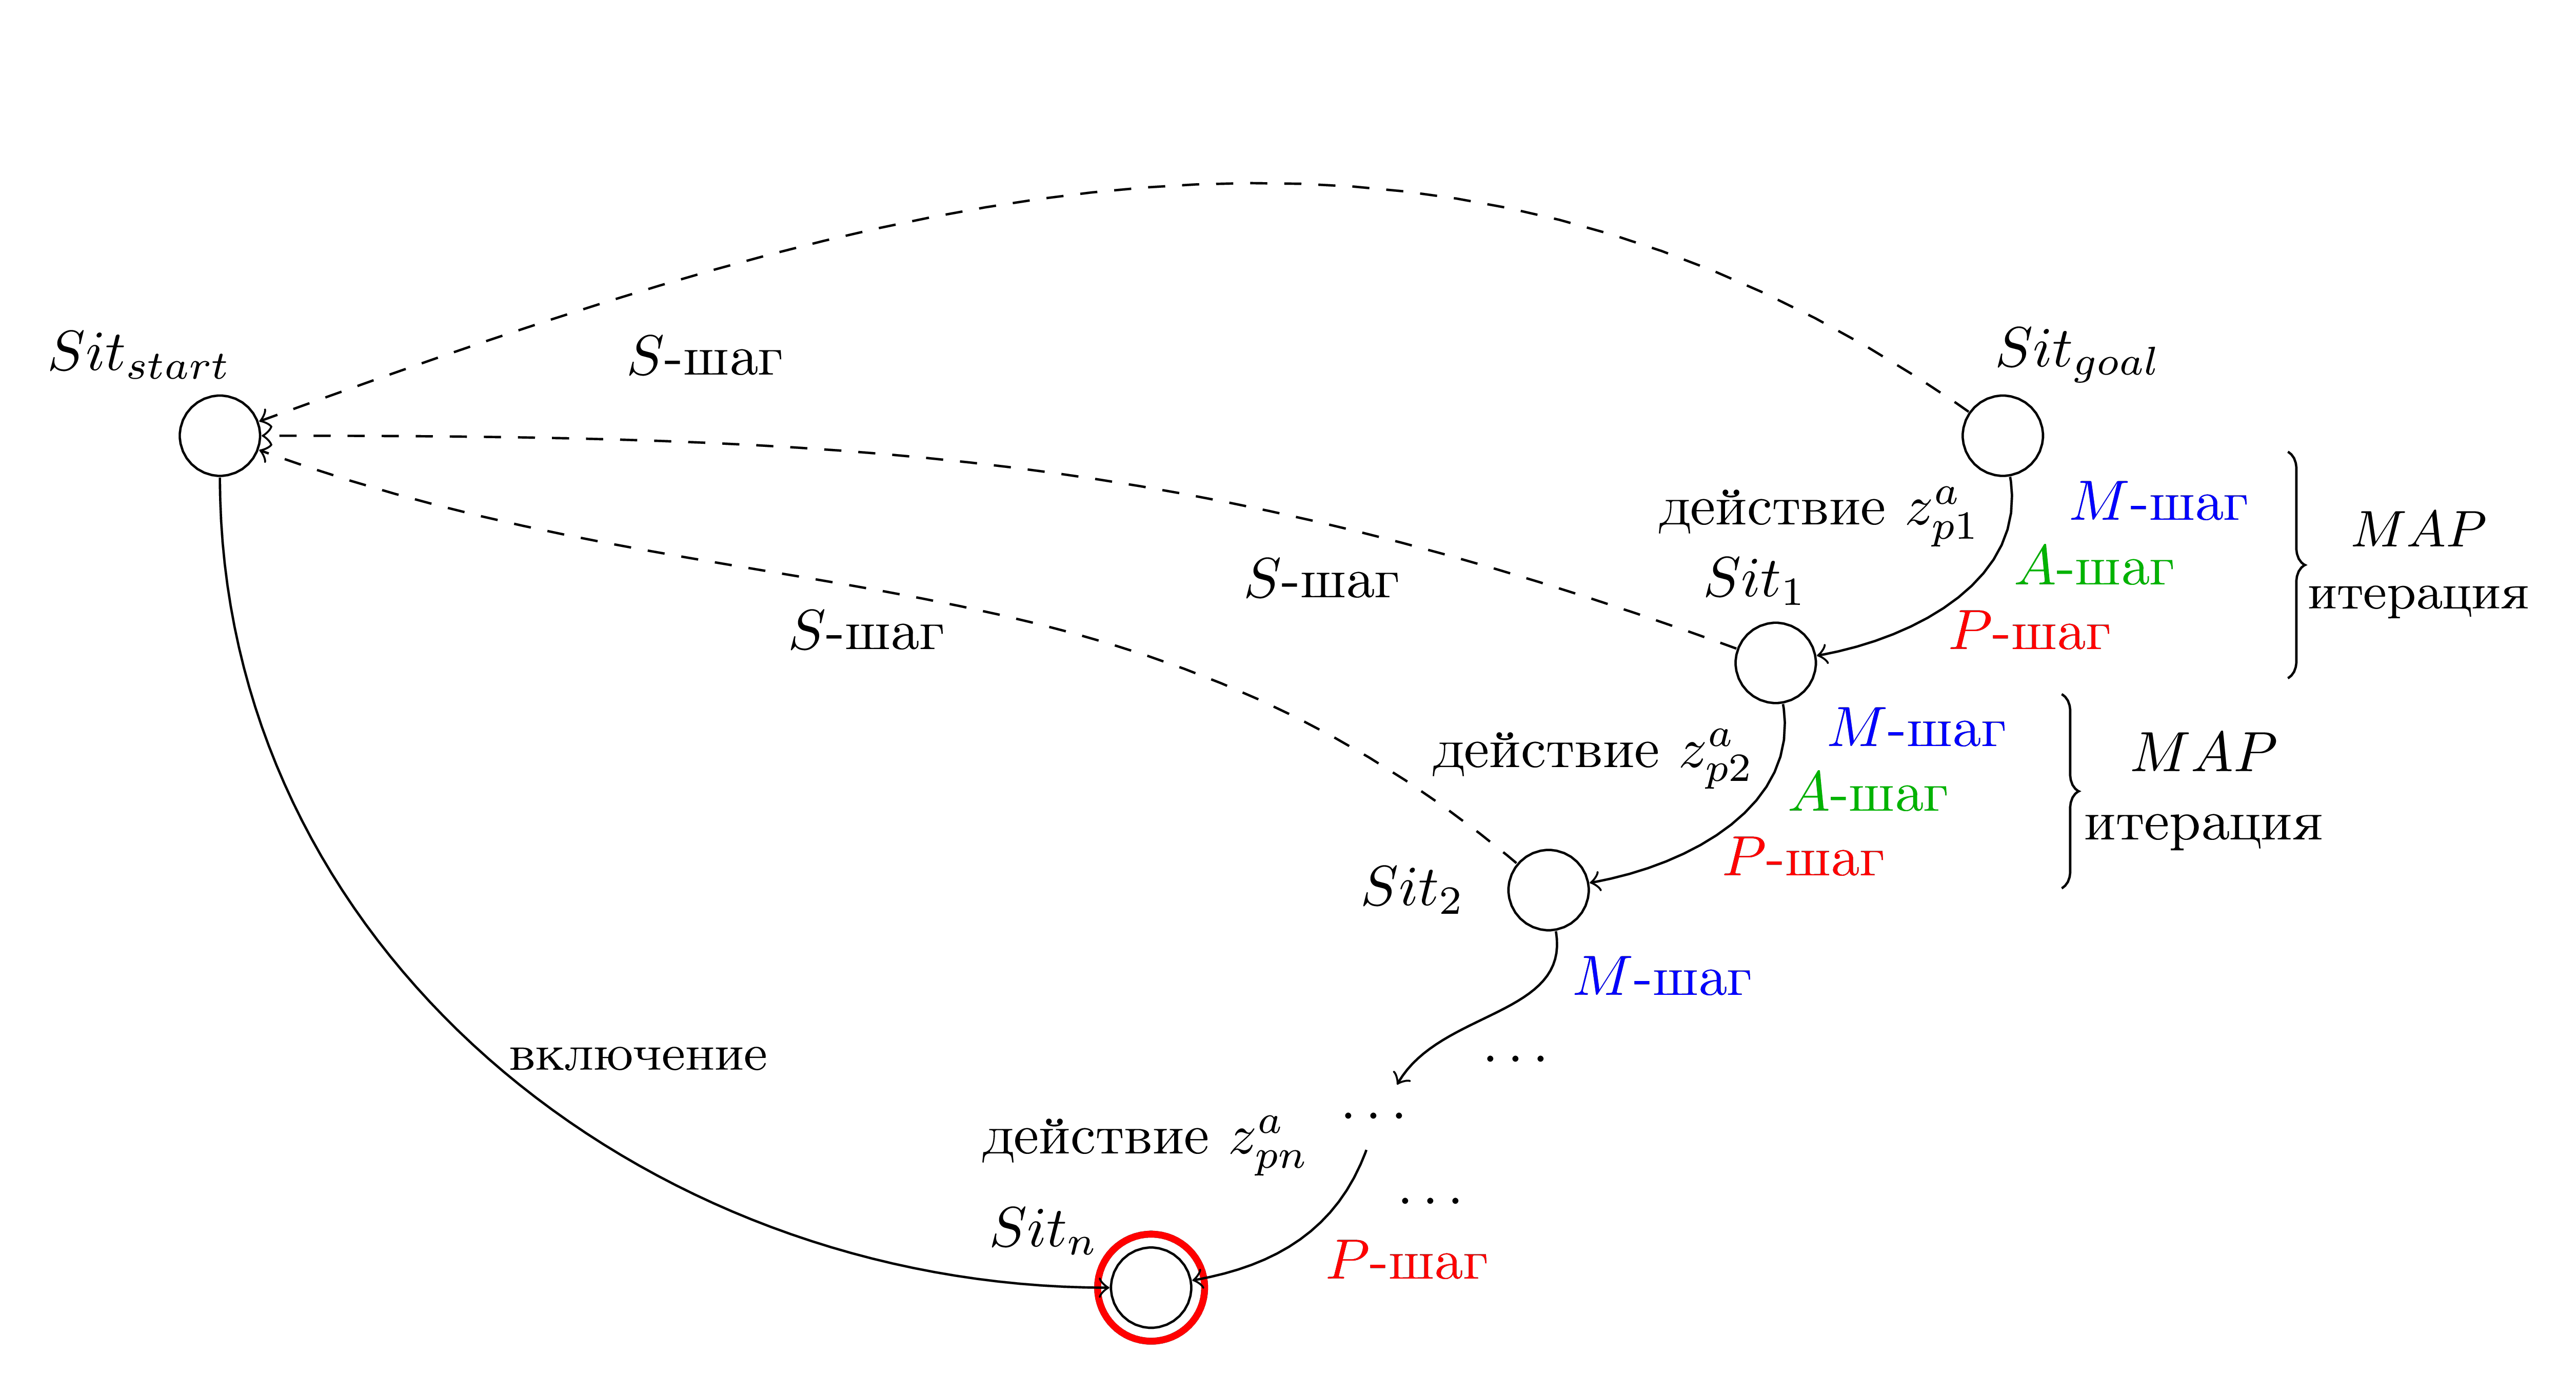
\includegraphics[width=0.5\textwidth]{algo/ru/map_ru}
					\end{center}
					\item Целеполагание.
					\begin{center}
						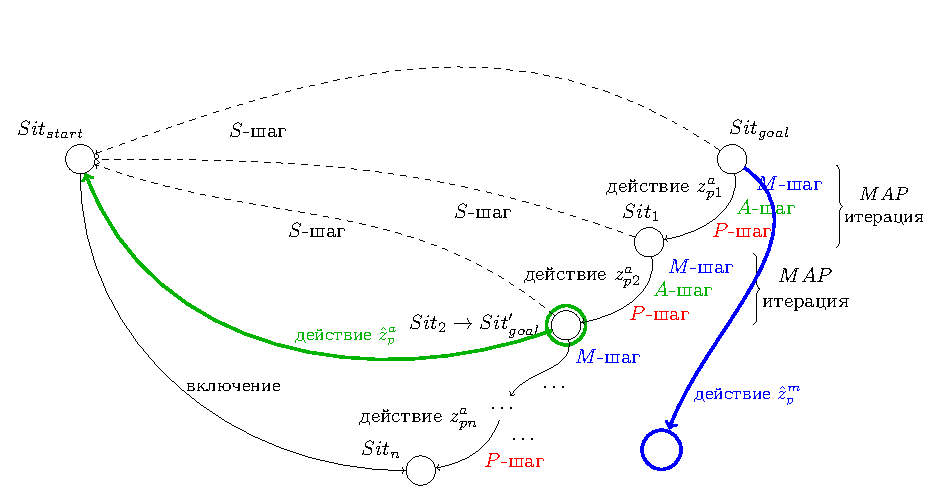
\includegraphics[width=0.5\textwidth]{algo/ru/gmap_ru}
					\end{center}
					\item Планирование коллективного поведения.
					\item Приобретение нового опыта.
				\end{itemize}
			\end{column}
		\end{columns}
		\textbf{Дальнейшее развитие}:
		\begin{itemize}
			\item Модели мета-когнитивных функций (эвристики в планировании, стратегии рассуждений) $\rightarrow$ перевод <<внешних>> функций во <<внутренние>> означенные действия.
			\item Развитие модели личностных смыслов $\rightarrow$ роль моторики и регуляции.
			\item Использование различных методов машинного обучения для формирования компонент знака (каузальных матриц) $\rightarrow$ обучение с подкреплением и анализ формальных понятий.
		\end{itemize}
	\end{frame}
		

%	\begin{frame}
%		\frametitle{Цели курса}
%		
%		\begin{columns}
%			\begin{column}{0.5\textwidth}
%				
%			\end{column}
%			\begin{column}{0.5\textwidth}
%				\begin{figure}
%					
\includegraphics[width=\textwidth]{logo}
%				\end{figure}
%			\end{column}
%		\end{columns}
%	\end{frame}
	%	\begin{frame}
	%		\frametitle{Цели курса}
	%		
	%		\begin{itemize}
	%			\item
	%		\end{itemize}
	%	\end{frame}
	
\end{document}
	
	
